%% LyX 2.4.0~RC3 created this file.  For more info, see https://www.lyx.org/.
%% Do not edit unless you really know what you are doing.
\documentclass[french]{beamer}
\usepackage[T1]{fontenc}
\usepackage[utf8]{inputenc}
\setcounter{secnumdepth}{3}
\setcounter{tocdepth}{3}
\usepackage{url}
\usepackage{amstext}
\usepackage{amssymb}
\usepackage{graphicx}
% import listings package
\usepackage{minted}

\synctex=1
\makeatletter

%%%%%%%%%%%%%%%%%%%%%%%%%%%%%% LyX specific LaTeX commands.
%% Because html converters don't know tabularnewline
\providecommand{\tabularnewline}{\\}

%%%%%%%%%%%%%%%%%%%%%%%%%%%%%% Textclass specific LaTeX commands.
% this default might be overridden by plain title style
\newcommand\makebeamertitle{\frame{\maketitle}}%
% (ERT) argument for the TOC
\AtBeginDocument{%
  \let\origtableofcontents=\tableofcontents
  \def\tableofcontents{\@ifnextchar[{\origtableofcontents}{\gobbletableofcontents}}
  \def\gobbletableofcontents#1{\origtableofcontents}
}

%%%%%%%%%%%%%%%%%%%%%%%%%%%%%% User specified LaTeX commands.

\AtBeginSection[]{
  \begin{frame}
  \vfill
  \centering
  \begin{beamercolorbox}[sep=8pt,center,shadow=true,rounded=true]{title}
    \usebeamerfont{title}\insertsectionhead\par%
  \end{beamercolorbox}
  \vfill
  \end{frame}
}

\setbeamertemplate{navigation symbols}{}

\addtobeamertemplate{navigation symbols}{}{%
    \usebeamerfont{footline}%
    \usebeamercolor[fg]{footline}%
    \hspace{1em}%
    \insertframenumber/\inserttotalframenumber
}



\makeatother


\begin{document}
\title{Introduction pratique aux modèles de language}
\author{Philippe Helluy}
\institute{IRMA, Université de Strasbourg, Inria Tonus}
\makebeamertitle
\begin{frame}{Plan}

\tableofcontents{}
\end{frame}
%

\section{Comment ça marche (en gros...)}
\begin{frame}{Très bref historique}
\begin{itemize}
\item Les réseaux de neurones artificiels existent depuis \textbf{longtemps}
(\cite{rosenblatt1958perceptron}, fin des années 50) 
\item Des hauts et des bas, puis \textbf{Yann LeCun} (\cite{lecun1989backpropagation},
reconnaissance d'écriture 1989)
\item \emph{Attention is all you need} \cite{vaswani2017attention}, invention
des \textbf{transformeurs} chez Google 
\item Sans une énorme \textbf{puissance} de calcul, ça ne marcherait pas.
\end{itemize}
\end{frame}
%
\begin{frame}{\emph{Completion is all you need}}
\begin{itemize}
\item Principe: on se donne un début de texte. Il faut prédire le mot suivant.
Exemple: \textquotedbl le chat mange le ...\textquotedbl{} (il faut
deviner \textquotedbl mulot\textquotedbl ).
\item Mots (ou \emph{tokens}):\\
\begin{tabular}{|c|c|c|c|c|c|}
\hline 
$t_{1}$ & $t_{2}$ & $t_{3}$ & $t_{4}$ & $t_{5}$ & $t_{6}=t_{m}$\tabularnewline
\hline 
\hline 
. & chat & le & mange & matou & mulot\tabularnewline
\hline 
\end{tabular}
\item Corpus: \textquotedbl le chat mange le mulot.\textquotedbl , \textquotedbl le
matou mange le mulot.\textquotedbl , \textquotedbl ..le chat mange.\textquotedbl ,
\textquotedbl ..le mulot mange.\textquotedbl , \textquotedbl ..le
matou mange.\textquotedbl , \emph{etc.}
\item Remarque: toutes les phrases ont $\ell=6$ mots (on complète avec
le mot bouche-trou \textquotedbl .\textquotedbl ).
\end{itemize}
\end{frame}
%
\begin{frame}{Numérisation}
\begin{itemize}
\item Codage: à chaque mot (ou \emph{token}) on associe un vecteur à $m=6$
dimensions{\footnotesize
\[
\text{"."}=\left[\begin{array}{c}
1\\
0\\
0\\
0\\
0\\
0
\end{array}\right],\quad\text{"chat"}=\left[\begin{array}{c}
0\\
1\\
0\\
0\\
0\\
0
\end{array}\right],\quad\text{"le"}=\left[\begin{array}{c}
0\\
0\\
1\\
0\\
0\\
0
\end{array}\right],\quad\text{\emph{etc.}}
\]
}{\footnotesize\par}
\item Plongement (\emph{embedding}) dans un espace de dimension $p$ plus
petite (pour tenir compte des synonymes, entre autres). Par exemple
$p=5$. Le plongement $E_{w_{0}}$ est une fonction de $\mathbb{R}^{m}$
à valeurs dans $\mathbb{R}^{p}$.
\item Chaque token $t_{i}$ est représenté par un vecteur $v_{i}$. Le vecteur
$w_{0}$ des paramètres du plongement est inconnu. 
\[
v_{i}=E_{w_{0}}(t_{i}).
\]
\end{itemize}
\end{frame}
%
\begin{frame}{Encodeur}
\begin{itemize}
\item Une phrase est donc représentée par un \textquotedbl tenseur\textquotedbl{}
de $\ell$ vecteurs numériques collés les uns derrière les autres:
\[
r_{0}=v_{i_{1}}v_{i_{2}}\ldots v_{i_{\ell}}
\]
C'est donc un objet dans un espace à $N=\ell\times p=30$ dimensions.
\item La phrase passe dans $k$ couches de transformeurs $T_{w_{i}}$, qui
sont des applications de $\mathbb{R}^{N}$ à valeurs dans $\mathbb{R}^{N}$
avec des vecteurs de paramètres inconnus $w_{i}$
\[
r_{i}=T_{w_{i}}(r_{i-1}),\quad i=1\ldots k.
\]
\item Plus on s'enfonce dans les couches, plus la représentation $r_{i}$
de la phrase initiale devient mystérieuse et abstraite. Le vecteur
$r_{k}$ contient l'information extraite par le réseau sur la phrase
initiale $r_{0}.$
\end{itemize}
\end{frame}

%
\begin{frame}{Décodeur}

Enfin, le décodeur va permettre de prédire un vecteur de probabilités
$p$ dans $\mathbb{R}^{m}$: $p_{i}$ est la probabilité que le mot
suivant soit $m_{i}$.
\[
p=D_{w_{k+1}}(r_{k}).
\]
En résumé (plus de précisions dans \cite{tunstall2022natural,vigon2023}):
\begin{center}
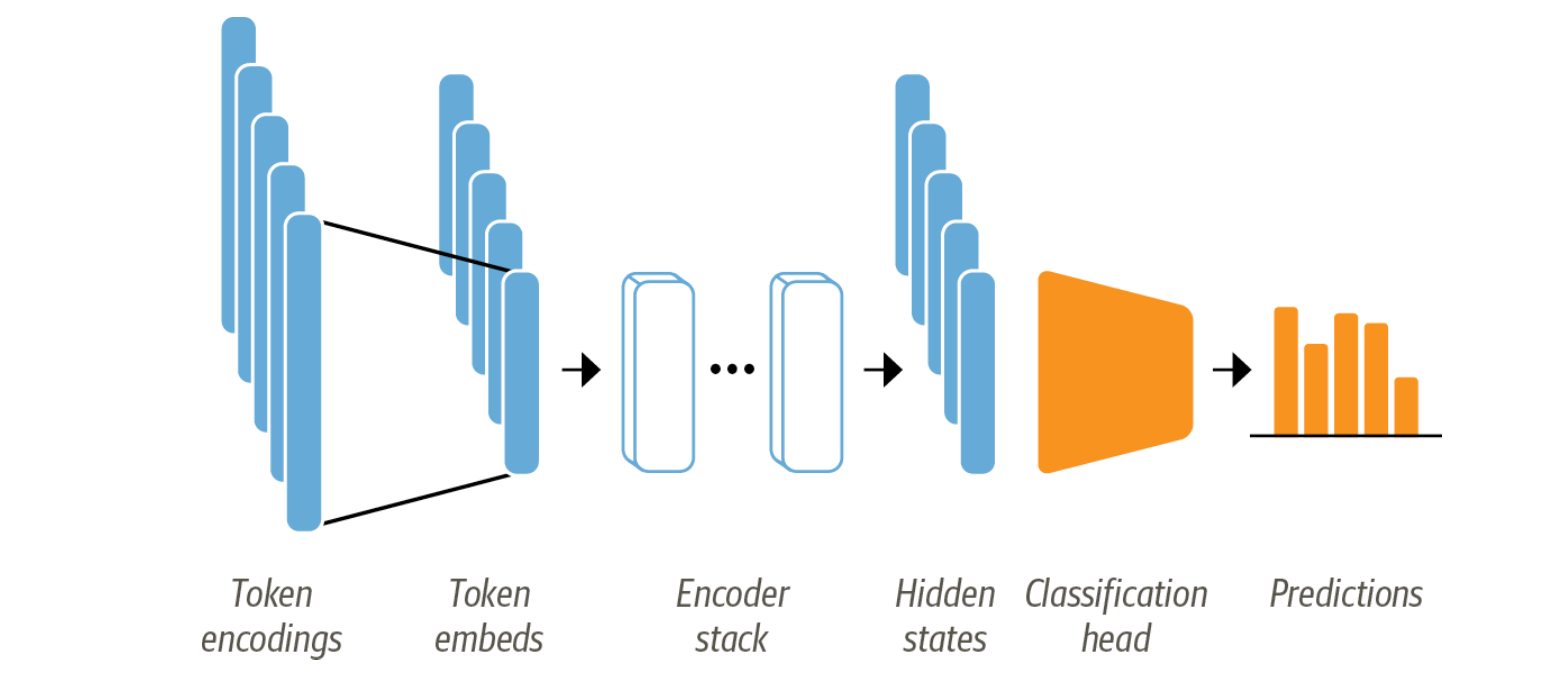
\includegraphics[width=0.9\textwidth]{../../IMPORTANT/Recherche/PyTorch/encode-decode}
\par\end{center}

\end{frame}
%
\begin{frame}{Entrainement}
\begin{itemize}
\item Choix de la forme des fonctions $E_{w_{0}}$, $T_{w_{i}}$, $D_{w_{k+1}}$:
c'est un compromis entre coût, efficacité, simplicité. C'est un art
autant que de la science pour l'instant.
\item Historiquement plusieurs formes possibles: CNN, RNN, LSTM, transformeurs.
Évolution fortement liée à la puissance de calcul disponible.
\item Le vecteur des paramètres $w$, de taille $s$ est \textbf{inconnu}.
\item L’entraînement consiste à optimiser le choix de ces paramètres pour
que le modèle retrouve au mieux les phrases du corpus.
\item C'est la partie la plus difficile du calcul, il faut un super-calculateur,
des processeurs spécialement conçus, ça coûte des millions d'euros.
\item Ordres de grandeurs pour GPT-3: $\ell=2000$, $m=50000$, $p=20000$,
$s=170$ milliard...
\end{itemize}
\end{frame}
%
\begin{frame}{Inférence}
\begin{itemize}
\item Une fois que les paramètres $w$ sont calculés, l'inférence est rapide.
\item On peut ré-entrainer un réseau pour une tâche spécifique, à coût réduit
(\emph{fine tuning}). Par exemple, Copilot et ChatGPT sont des versions
spécialisées de GPT-3.
\item Le \textit{pre-prompt} est essentiel pour obtenir des résultats de
qualité.
\item Pour des raisons de coût de calcul, \textbf{ChatGPT n'apprend pas
en temps réel}. Sa mémoire à court terme est donc limitée à quelques
milliers de mots.
\end{itemize}
\end{frame}
%
\begin{frame}{Exemple avec PyTorch}
\begin{itemize}
\item PyTorch est une bibliothèque logicielle libre développée par la société
Huggingface pour manipuler des réseaux de neurones.
\item Exemple minimal d'utilisation.
\end{itemize}
\end{frame}

\section{Fine tuning of Qwen LLM for time series annotation}
\begin{frame}[fragile]{Objectives}

\begin{itemize}
\item Teach a small LLM (Qwen2.5 0.5 billions parameters) to describe a
time series
\item Example of prompt:\\
\begin{minted}[fontsize=\tiny]{markdown}
Describe the time series in three sentences.
First sentence: describe trend (increasing/decreasing/flat).
Second sentence: noise intensity (low/medium/high).
Third sentence: approximate localisation of global maximum (beginning/middle/end)
and global minimum (beginning/middle/end).
Put the description in a JSON format with the following pattern
<json>{ "trend": <sentence1>,
"noise": <sentence2>,
"extrema": <sentence3> }
</json>
Series: [02, 01, 00, 03, ... ]
\end{minted}
\item Tokenization is essential: the values in the series are scaled to the range 00..99.
\end{itemize}
\end{frame}

\begin{frame}[fragile]{Necessity of training}

\begin{itemize}
\item Small LLM fails to answer properly. It generates total garbage.
\item Example of output:\\
\begin{minted}[fontsize=\tiny]{markdown}
series name: \"series\"
time interval: 1 day
``` To provide a detailed analysis of the given time series data, I will break it down into its components:
### Time Series Description:
The provided time series consists of daily values for several variables over a period of one year (assuming 365 days).
### Trend Analysis:
- **Increase**: The values increase steadily from 01 to 04, then decrease again.
- **Decrease**: The values decrease from 04 onwards
...
\end{minted}
\item Let's try to improve this with supervised fine tuning
\end{itemize}
\end{frame}

\begin{frame}[fragile]{Practical methodology}

\begin{itemize}
\item Generate a dataset of correct examples with a large LLM (Mistral, ChatGPT, etc.)
\item Apply a supervised fine tuning (SFT) procedure on a small LLM from this dataset.
\item In order to reduce the cost we adopt a LoRA approach. \footnote{The LoRA (Low-Rank Adaptation) approach in supervised fine-tuning (SFT) freezes the original model weights and injects small trainable low-rank matrices into certain layers (typically linear projections in attention/FFN). This drastically reduces the number of parameters that need updating, making fine-tuning large models much more memory- and compute-efficient while still achieving strong adaptation.}
\item Now go to \url{https://github.com/phelluy/DLAA_2025} and follow the README file.
\end{itemize}
\end{frame}
%


\end{document}
